\documentclass[border=10pt]{standalone}

\usepackage[utf8]{inputenc}                                 % Codificação do documento
\usepackage[T1]{fontenc}                                    % Seleção de código de fonte
\usepackage{microtype}                                      % Melhora a justificação do documento
\usepackage{lmodern}                                       % Usa a fonte Latin Modern
\usepackage{ae, aecompl}                                    % Fontes de alta qualidade

\usepackage{amsmath}
\usepackage{verbatim}
\usepackage{tikz}
\usetikzlibrary{arrows,calc,positioning,shadows.blur,decorations.pathreplacing}
\usepackage{etoolbox}

\begin{document}
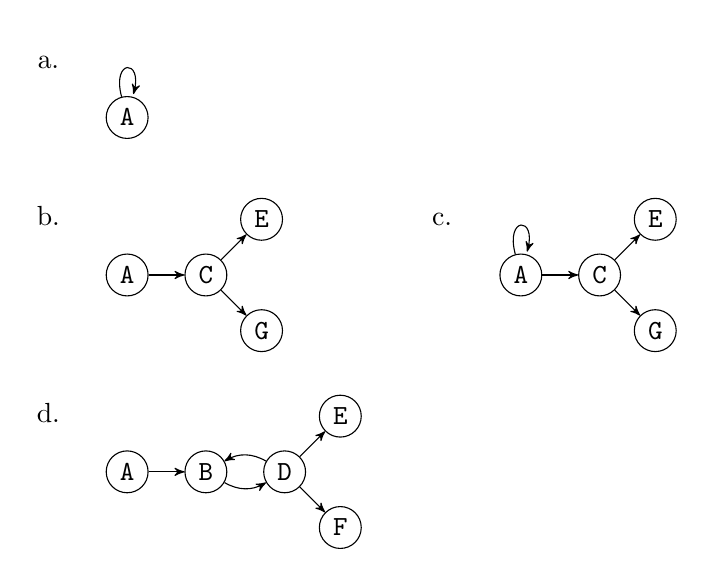
\begin{tikzpicture}
[
	              y = -1cm,
	           ->, >= stealth',
	  node distance = 2cm,
	  vertex/.style = { draw=black, circle, inner sep=2.5pt },
	toplabel/.style = { label, anchor=south }
]
	% first trace
	% nodes
	\node (T1) at (-1,-0.5) [toplabel] {a.};
	\node (A) at (0,0)    [vertex]   {\texttt{A}};

	% edges
	\draw [->] (A) edge [loop above] (A);

	% second trace
	% nodes
	\node (T2) at (-1,1.5)        [toplabel] {b.};
	\node  (A) at (0,2)           [vertex]   {\texttt{A}};
	\node  (C) at (1,2)           [vertex]   {\texttt{C}};
	\node  (E) at (1.7071,1.2929) [vertex]   {\texttt{E}};
	\node  (G) at (1.7071,2.7071) [vertex]   {\texttt{G}};

	% edges
	\draw [->] (A) edge (C) (C) edge (E) (C) edge (G);

	% third trace
	% nodes
	\node (T3) at (4,1.5)         [toplabel] {c.};
	\node  (A) at (5,2)           [vertex]   {\texttt{A}};
	\node  (C) at (6,2)           [vertex]   {\texttt{C}};
	\node  (E) at (6.7071,1.2929) [vertex]   {\texttt{E}};
	\node  (G) at (6.7071,2.7071) [vertex]   {\texttt{G}};

	% edges
	\draw [->] (A) edge [loop above] (A) (A) edge (C) (C) edge (E) (C) edge (G);

	% fourth trace
	% nodes
	\node (T4) at (-1,4)          [toplabel] {d.};
	\node  (A) at (0,4.5)         [vertex]   {\texttt{A}};
	\node  (B) at (1,4.5)         [vertex]   {\texttt{B}};
	\node  (D) at (2,4.5)         [vertex]   {\texttt{D}};
	\node  (E) at (2.7071,3.7929) [vertex]   {\texttt{E}};
	\node  (F) at (2.7071,5.2071) [vertex]   {\texttt{F}};

	% edges
	\draw [->] (A) edge (B) (B) edge [bend right] (D) (D) edge [bend right] (B) (D) edge (E) (D) edge (F);
\end{tikzpicture}
\end{document}